\chapter{CRE}
\label{cap4}

Estes parâmetros são atributos específicos de uma frente de onda hipotética atribuídos a cada evento de reflexão
primária de afastamento nulo: O raio de curvatura RNIP e o ângulo de emergência $\beta_0$. Esta onda hipotética é
a onda NIP (Hubral, 1983)

Hubral, P.
Computing true-amplitude reflections in a laterally inhomogeneous earth
Geophysics 48 1052-1063



O método do elemento de reflexão comum (CRE) é uma alternativa interessante para os métodos usuais de empilhamento PMC ou
migração para a seção de afastamento nulo. No entanto não requere conhecimento do modelo geral em subsuperfície, apenas
o conhecimento da velocidade próximo a superfície é necessário a priori.
O método ERC é baseado somente em considerações cinemáticas em 2D e não é
um processo que preserva as amplitudes.

A principal e provavelmente mais importante vantagem do método ERC em comparação com o empilhamento PMC convencional
é que este proporciona, além da seção empilhada, parâmetros importantes para a construção do macromodelo de 
velocidades que pode inclusive variar lateralmente.

Os parâmetros $R_{NIP}$ e $\beta_0$ atribuídos aos pontos $P_0(x_0,\tau_0)$ são obtidos a partir do método ERC.
Estes dois atributos podem ser utilizados para estimar o macromodelo de velocidades.
O método ERC, além de ser um processo para simular as seções de afastamento nulo sem o conhecimento prévio
do macromodelo de velocidades, também permite determinar os atributos da onda NIP $(R_{NIP},\beta_0)$
que combinado com outras estratégias permitem estimar o macromodelo de velocidades.

As principais características do método ERC:
(a) A construção da seção de afastamento nulo a partir de um conjunto de seções de afastamento constante
com apenas uma estimativa da velocidade próxima da superfície.
(b) A determinação dos parâmetros $(R_{NIP},\beta_0)$ para as reflexões de afastamento nulo na seção empilhada.
Estes atributos podem ser utilizados com técnicas de inversão para estimar o macromodelo de velocidades.

A idéia principal do método ERC é, usando a fórmula do tempo de trânsito ERC, no modelo auxiliar, dado um intervalo
de busca para os parâmetros $R_{NIP}$ e $\beta_0$, encontrar a frente de onda NIP que melhor se ajusta aos dados.
Este processo é semelhante a análise sobretempo normal convencional, todavia enquanto esta análise é feita no
domínio PMC, o método ERC é feito no domínio ERC construído durante o processo, o parâmetro otimizado $R_{NIP}$,$\beta_0$
é especificado a partir da análise de coerência nos dados.


\begin{figure}[htb]
\caption{Representação esquemática de um arranjo ERC para um refletor circular de raio $R$ e profundidade
mínima $D$: A família ERC é formada pelos pares $s_i$-$r_i$ (fonte-receptor) que possuem o mesmo ponto de
reflexão em subsuperfície ($NIP$). A família ERC pode ser entendida a partir de uma fonte pontual explosiva
no ponto $NIP$, que ao ser ativada forma uma frente de onda $NIP$ que atinge a superfície em um PMC central 
$m_0$ com raio de curvatura $R_{NIP}$ e ângulo de incidência $\beta_0$.}
\begin{center}
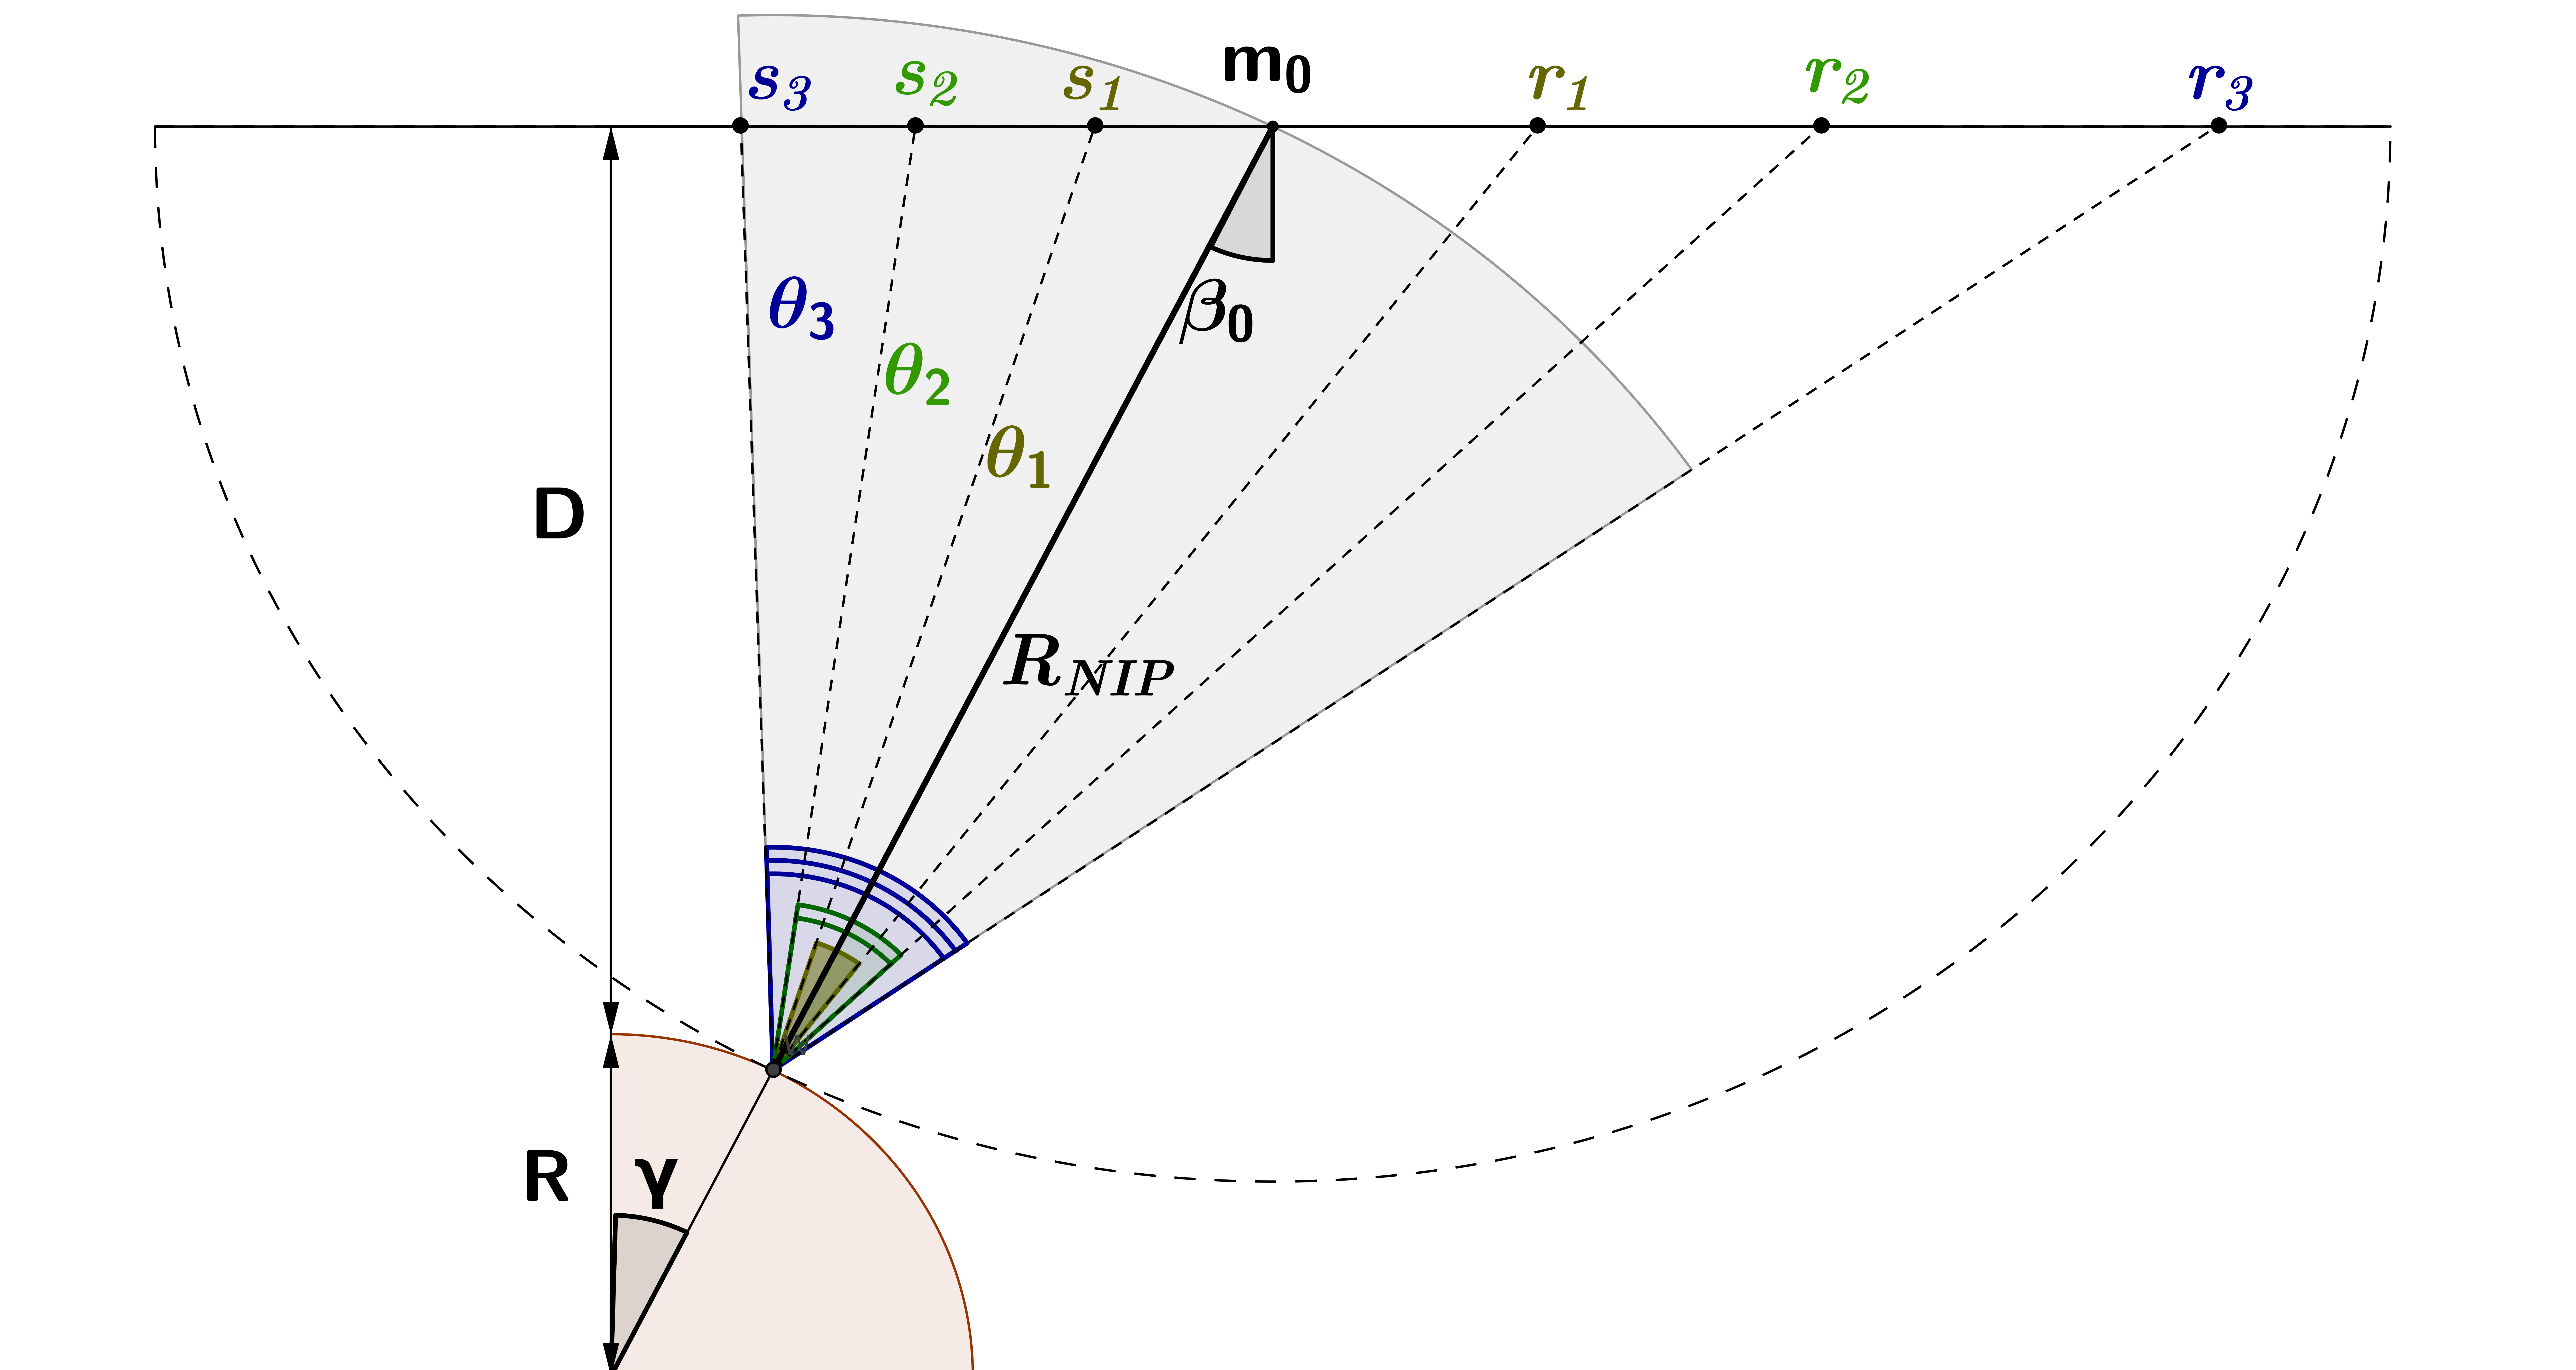
\includegraphics[scale=0.3]{cre.png}
\vspace{-0.3cm}
\end{center}
\begin{center}
 Fonte: Do Autor.
\end{center}
\label{fig:4.1}
\end{figure}


\begin{figure}[htb]
\caption{Representação esquemática das coordenadas do ERC sobre o modelo do refletor circular da Figura \ref{fig:4.1}:
Modificamos a posição do PMC central $m_0$ variando o ângulo $\gamma$ no modelo do refletor circular.
Ao variarmos o ângulo $\theta$, mantendo $\gamma$ constante, obtemos os pares $s_i$-$r_i$ (fonte-receptor)
dentro da família
ERC, as posições $h$ (meio afastamento) e $m$ (PMC) são obtidas para cada par fonte-receptor.
Cada curva colorida representa uma posição
diferente de $m_0$, um valor diferente de $R_{NIP}$ e $\beta_0$, e uma família ERC diferente.}
\begin{center}
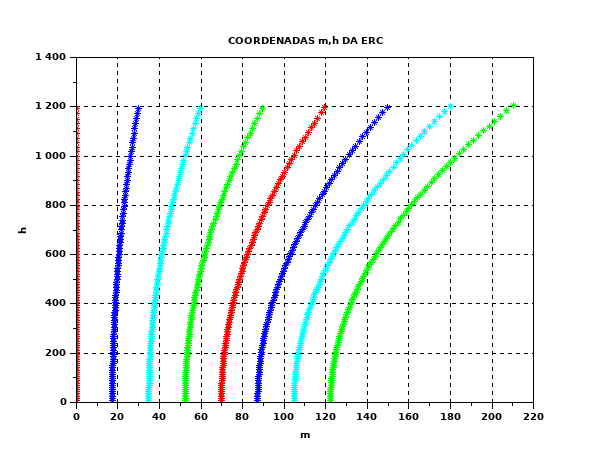
\includegraphics[scale=0.5]{coordenadas_CRE.png}
\vspace{-0.3cm}
\end{center}
\begin{center}
 Fonte: Do Autor.
\end{center}
\label{fig:4.2}
\end{figure}





O parâmetro de assimetria desenpenha um papel importante na seleção de pares fonte-receptor para os quais
o correspondente raio de reflexão refletem no mesmo ponto \cite{tygel}.


